\documentclass[10pt]{article}
\usepackage{parskip}
\usepackage[utf8]{inputenc}
\usepackage[left=2.00cm, right=2.00cm, top=2.00cm, bottom=2.00cm]{geometry}
\usepackage[spanish]{babel}
\usepackage{graphicx,subfig}
\usepackage{fancyhdr}
\graphicspath{{Imagenes/}}
\usepackage{enumerate} 
\usepackage{multicol}
\begin{document}


\pagestyle{fancy}
\cfoot{}


%Cabeceras
\rhead{Multímetro.}
\lhead{}

%Portada
\begin{titlepage}
	\newgeometry{
		left=25mm,
		right=25mm,
		top=5mm,
		bottom=30mm,
		headheight = 0 mm
	}

	\begin{figure}[t]
		\subfloat{
\includegraphics[width=0.15\textwidth]{Logo_IPN}}
		\hspace{0.6\textwidth}
		\subfloat{
\includegraphics[width=0.22\textwidth]{LogoEsime}}
	\end{figure}

	\centering
	{\bfseries\Huge Instituto Politécnico Nacional. \par}
	\vspace{1cm}
	{\scshape\Large Ingeniería en Comunicaciones y Electrónica. \par}
	\vspace{0.3cm}
	{\scshape\Large Laboratorio de Electricidad y Magnetismo.  \par}
	\vspace{1cm}
	{\scshape\Huge El Universo de las Mediciones Eléctricas. \par}
	\vspace{1cm}
	{\itshape\Large Multímetro. \par}
	{\Large 2CM13\par}
	\vfill
	{\Large Autores: \par}
	{\Large Daniela Elizabeth Pérez Vargas. \par}
	{\Large Jesús Martinez Amac. \par}
	{\Large José Emilio Hernández Huerta. \par}
	{\Large Nataly Bejarano Garduño.\par}
	{\Large Uriel Grimaldi Díaz.  \par}
	\vfill
	{\Large Mayo 2023. \par}

\end{titlepage}

\tableofcontents
\newpage

\section{Resumen.}
En la presente práctica, se desarrolla el uso del multímetro con enfásis en las funciones de medición de resistencia, continuidad, vóltmetro (Corriente Directa y Corriente Alterna) y Amperímetro. 

\begin{multicols}{2}

\section{Objetivo.}

El alumno será capaz de describir las características y funcionamiento del multímetro así como manejar correctamente dicho instrumento para realizar mediciones de las 3 magnitudes eléctricas fundamentales (Resistencia, Potencial eléctrico y Corriente eléctrica).

\section{Introducción.}

La herramienta fundamental del técnico o ingeniero especializado en la manipulación de componentes electrónicos es el multímetro, dicha herramienta permite al profesional obtener mediciones de magnitudes eléctricas que le puedan resultar útiles,
estas magnitudes suelen ser , la resistencia eléctrica, el potencial eléctrico, la corriente eléctrica,frecuencia, inductancia, capacitancia además de otras utilidades como la continuidad y la prueba de diodos.

\section{Marco teórico.}

\subsection{El multímetro.}
Se denomina multimetro al instrumento que es capaz de realizar las funciones de voltímetro, amperímetro y óhmetro. Los multimetros digitales suelen incorporar funciones adicionales como capacítometro, frecuenciometro, medida de hfe (ganancia) de transistores, para medir 
temperaturas sobre superficies además de otras utilidades como la continuidad eléctrica y la prueba de diodos.

Con los multímetros digitales no solo es posible realizar medidas de voltaje y de corrientes continuas, si no que también nos permiten medir el voltaje de corrientes alternas.

Un multímetro está formado por distintos bloques funcionales que forman las "etapas" de tratamiento de la señal a medir.

\begin{center}
	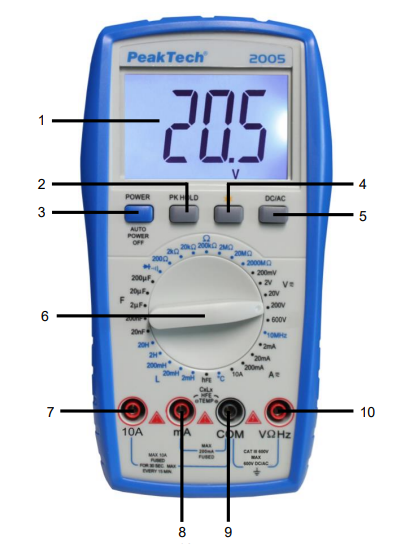
\includegraphics[scale = 0.5]{Imagenes/Marco/Multimetro.PNG}\\
	\begin{enumerate}
		\item Pantalla LCD
		\item Tecla PK Hold.
		\item Tecla de encendido y apagado.
		\item Tecla de retroiluminación.
		\item Tecla Corriente Directa / Corriente Alterna.
		\item Selector.
		\item Conector de entrada 10 A.
		\item Conector de entrada mA/temp.
		\item Conector de entrada COM.
		\item Conector de entrada V/$\Omega$/Hz.
	\end{enumerate}
\end{center}

Un consejo relevante cuando se usan instrumentos analógicos es que siempre conviene medir lo máximo posible el fondo de escala para reducir el error en la medición.

\subsection{Antes de usar un multímetro.}
Dentro de las comprobaciones de rutina tenemos , primeramente, asegurarnos de que el multímetro tenga buena carga de batería, una forma de saber si tiene una carga adecuada de batería si el multímetro no posee medidor de batería es hacer una prueba de continuidad, si el sonido
es débil es probable que el multímetro requiera de batería.

También tenemos que verificar que el fusible de protección del multímetro no esté cortado, generalmente este fusible se encuentra en la parte trasera del multímetro. Verificamos de igual manera que las puntas se encuentren en buenas condiciones y por último, una correcta medida se hace
sin tocar las puntas metalicas , solo sosteniendo las puntas de medición por su mango de plástico.

\subsection{Como utilizar el multímetro.}

A continuación se detallaran las recomendaciones e instrucciones para utilizar correctamente el multímetro para leer las 3 magnitudes fundamentales (Potencial eléctrico,corriente y resistencia).
\subsubsection{Potencial eléctrico.}

Siga las recomendaciones del manual de usuario sobre el máximo de Potencial Eléctrico soportado por su multimetro.
\begin{enumerate}
	\item Coloque el selector en la posición adecuada. Seleccione el rango según se necesite, si no conoce el valor apróximado a medir, inicie primero en la posición de mayor escala y vaya reduciendo según lo pida la lectura.
	\item Conecte la punta de medición negra a la terminal COM y la punta roja a la terminal V/$\Omega$/Hz.
	\item Conecte las puntas de medición a la fuente que desee medir.
\end{enumerate}

Como recomendación adicional, es importante no girar el selector a otro rango ya que podría dañar los componentes del medir.
\subsubsection{Corriente eléctrica.}

Primeramente dee conectar el medidor en serie con el circuito.

Las terminales que permiten medir Corriente eléctrica suelen estar protegidas por fisibles. Existe un riesgo de incendio o cortocircuito si se aplica un potencial eléctrico con la capacidad de llevar altas corrientes, lo que puede malograr el dispositivo.

Para medir la corriente, abra el circuito y conecte las puntas a los puntos de los dos circuitos de conexión. Nunca conecte las puntas a una sola fuente en paralelo ya que puede quemar el fusible o dañar el circuito que está bajo prueba.

Por último, es importante revisar las especificaciones del multimetro utilizado para saber así su rango de operatividad.

\begin{enumerate}
	\item Coloque el selector en el rango A necesitado. Si no lo conoce, inicie desde una posición alta y vaya desendiendo.
	\item Conecte la punta negra al terminar COM y la punta roja a la terminal mA o 10A según el rango necesitado.
	\item Corte la corriente del circuito bajo prueba y luego abra el circuito en el punto apropiado.
	\item Conecte las puntas en serie con el circuito. 
	\item Conecte la alimentación y lea la corriente.
\end{enumerate}
\subsubsection{Resistencia.}

Nunca conecte las puntas de prueba a una fuente cuando haya seleccionado la función "Ohms" y conectado las puntas al terminal V/$\Omega$/Hz.

Asegúrese que el circuito no esté conectado a ninguna fuente de alimentación y que cualquier condensador asociado a él esté completamente descargado.

\begin{enumerate}
	\item Coloque el selector en el rango de Ohm deseado.
	\item Conecte la punta negra a la terminal COM y la punta roja a la terminal V/$\Omega$/Hz.
	\item Conecte ambas puntas al dispositivo que desee medir.
\end{enumerate}

\subsection{Ley de Ohm.}

La ley de Ohm formulada por el físico alemán Georg Simon Ohm establece que cuando por un circuito eléctrico que ofrece cierta
resistencia R al paso de la corriente que esté a circulando una intensidad I, se produce
una diferencia de potencial $\Delta$ V entre sus extremos que obedece a la siguiente expresión:

\begin{equation}
	\Delta V = IR
\end{equation}

La importancia de la Ley de Ohm radica en que permite calcular y predecir el comportamiento de los circuitos eléctricos.

Algunos ejemplos de su uso y aplicación son los siguientes:

\begin{enumerate}
	\item Cálculo de corriente, potencial eléctrico o resistencia desconocidos: Si conoces dos de los valores (corriente, potencial eléctrico o resistencia) en un circuito, puedes utilizar la Ley de Ohm para calcular el tercer valor desconocido.
	\item Dimensionar componentes y calcular resistencias apropiadas para lograr el flujo de corriente deseado en un circuito.
	\item Evaluar si un circuito cumple con los límites de corriente y potencial eléctrico especificados por los dispositivos.
\end{enumerate}
\section{Descripción de materiales.}

\begin{center}

	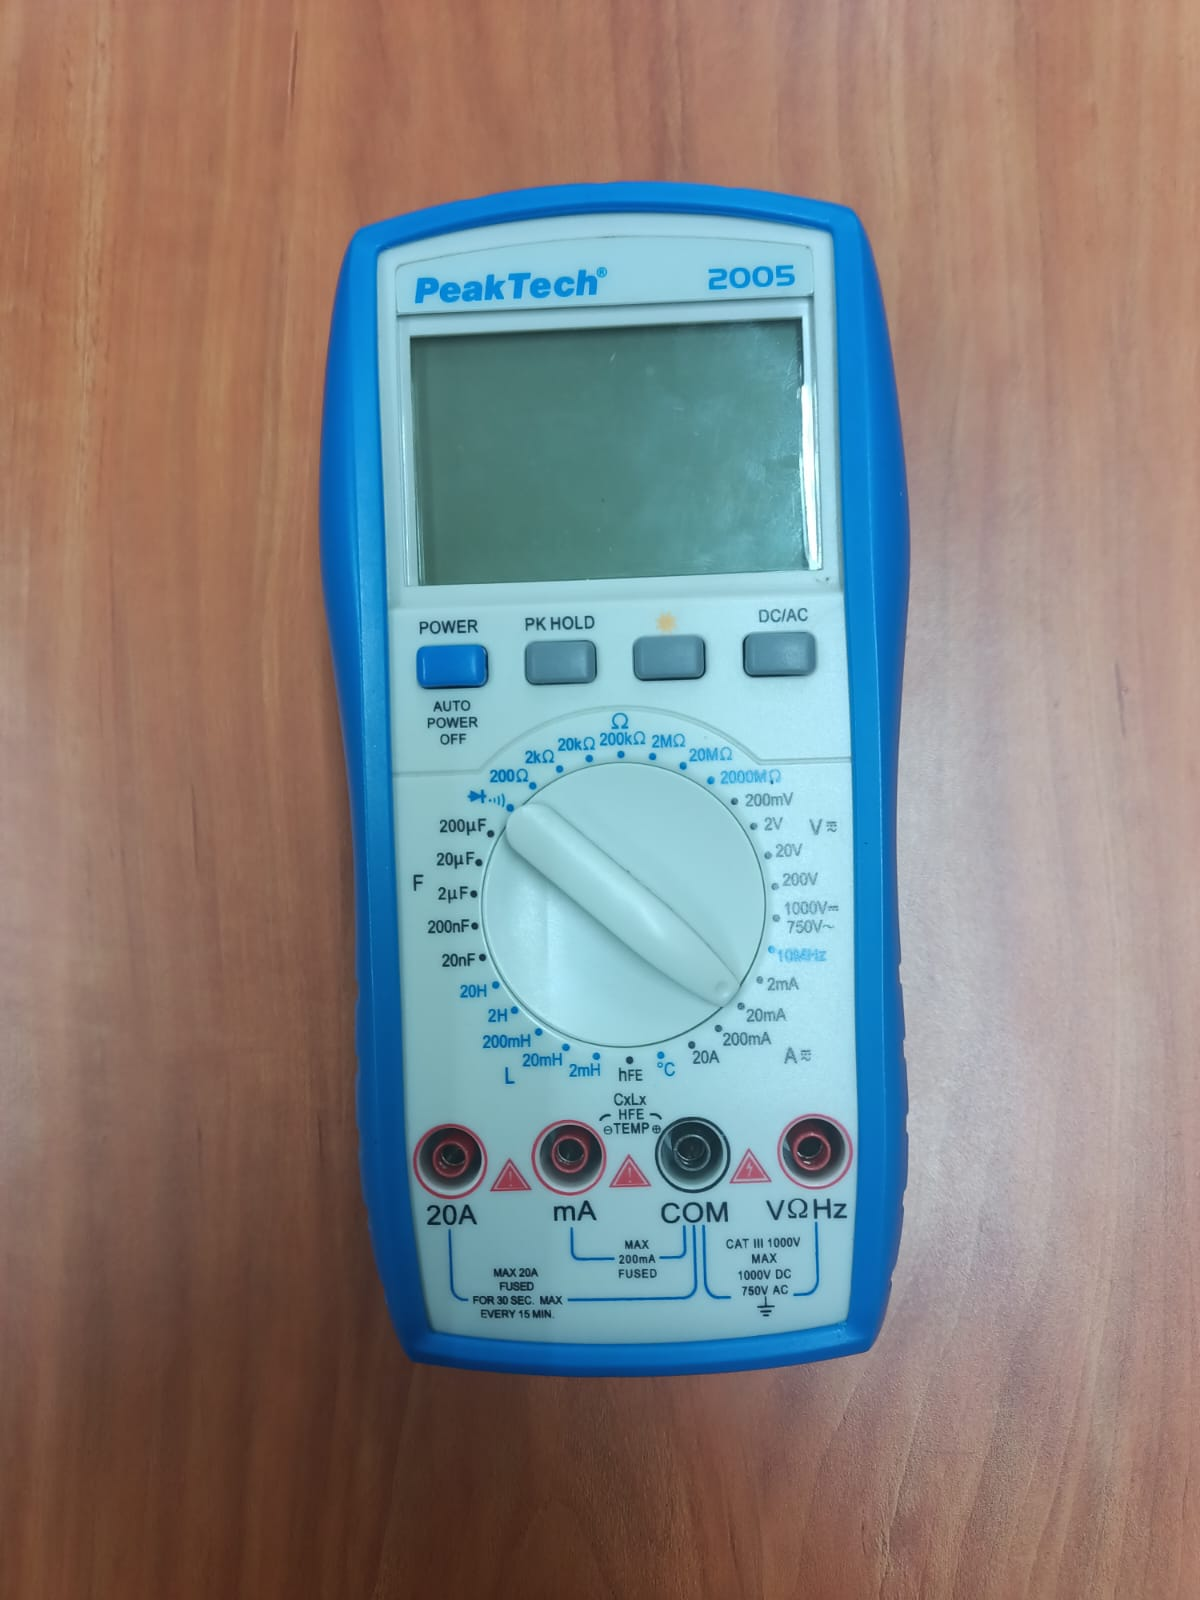
\includegraphics[scale = 0.1]{Imagenes/Material/MultiD.jpeg}\\
	Multímetro Digital.

	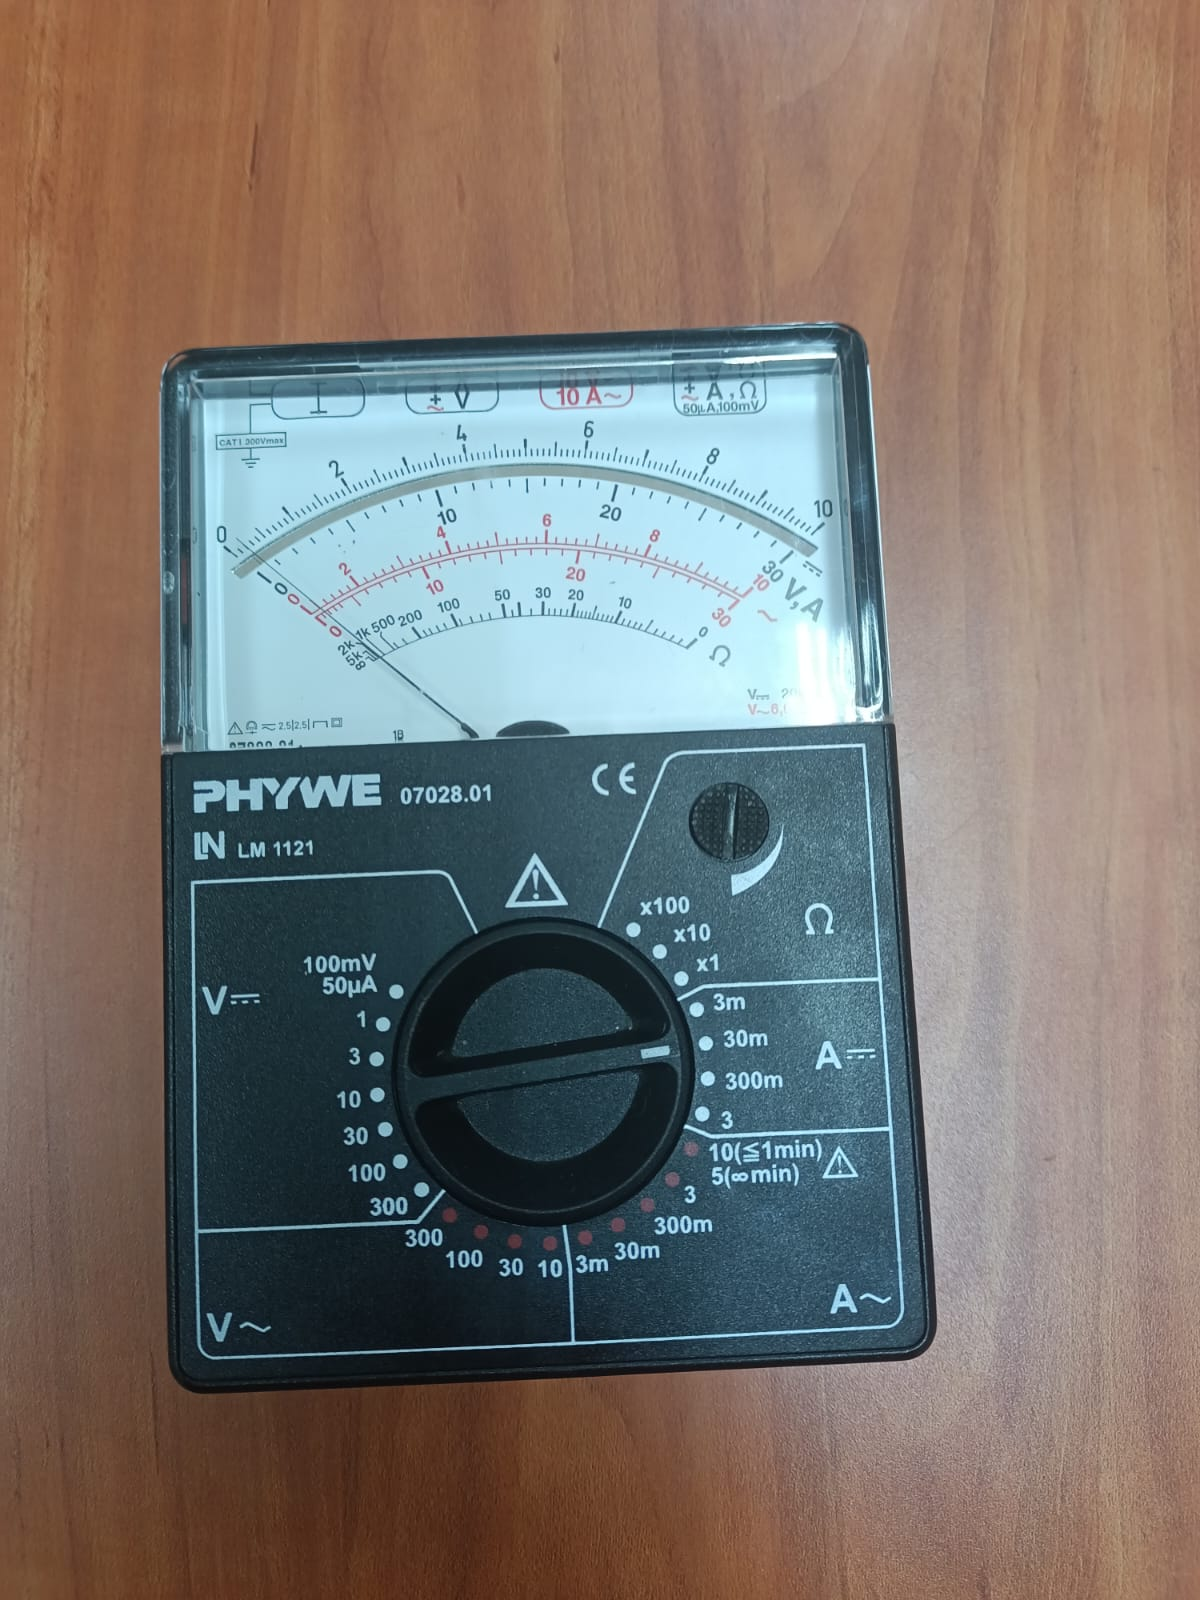
\includegraphics[scale = 0.1]{Imagenes/Material/MultiA.jpeg}\\
	Multímetro Analógico.

	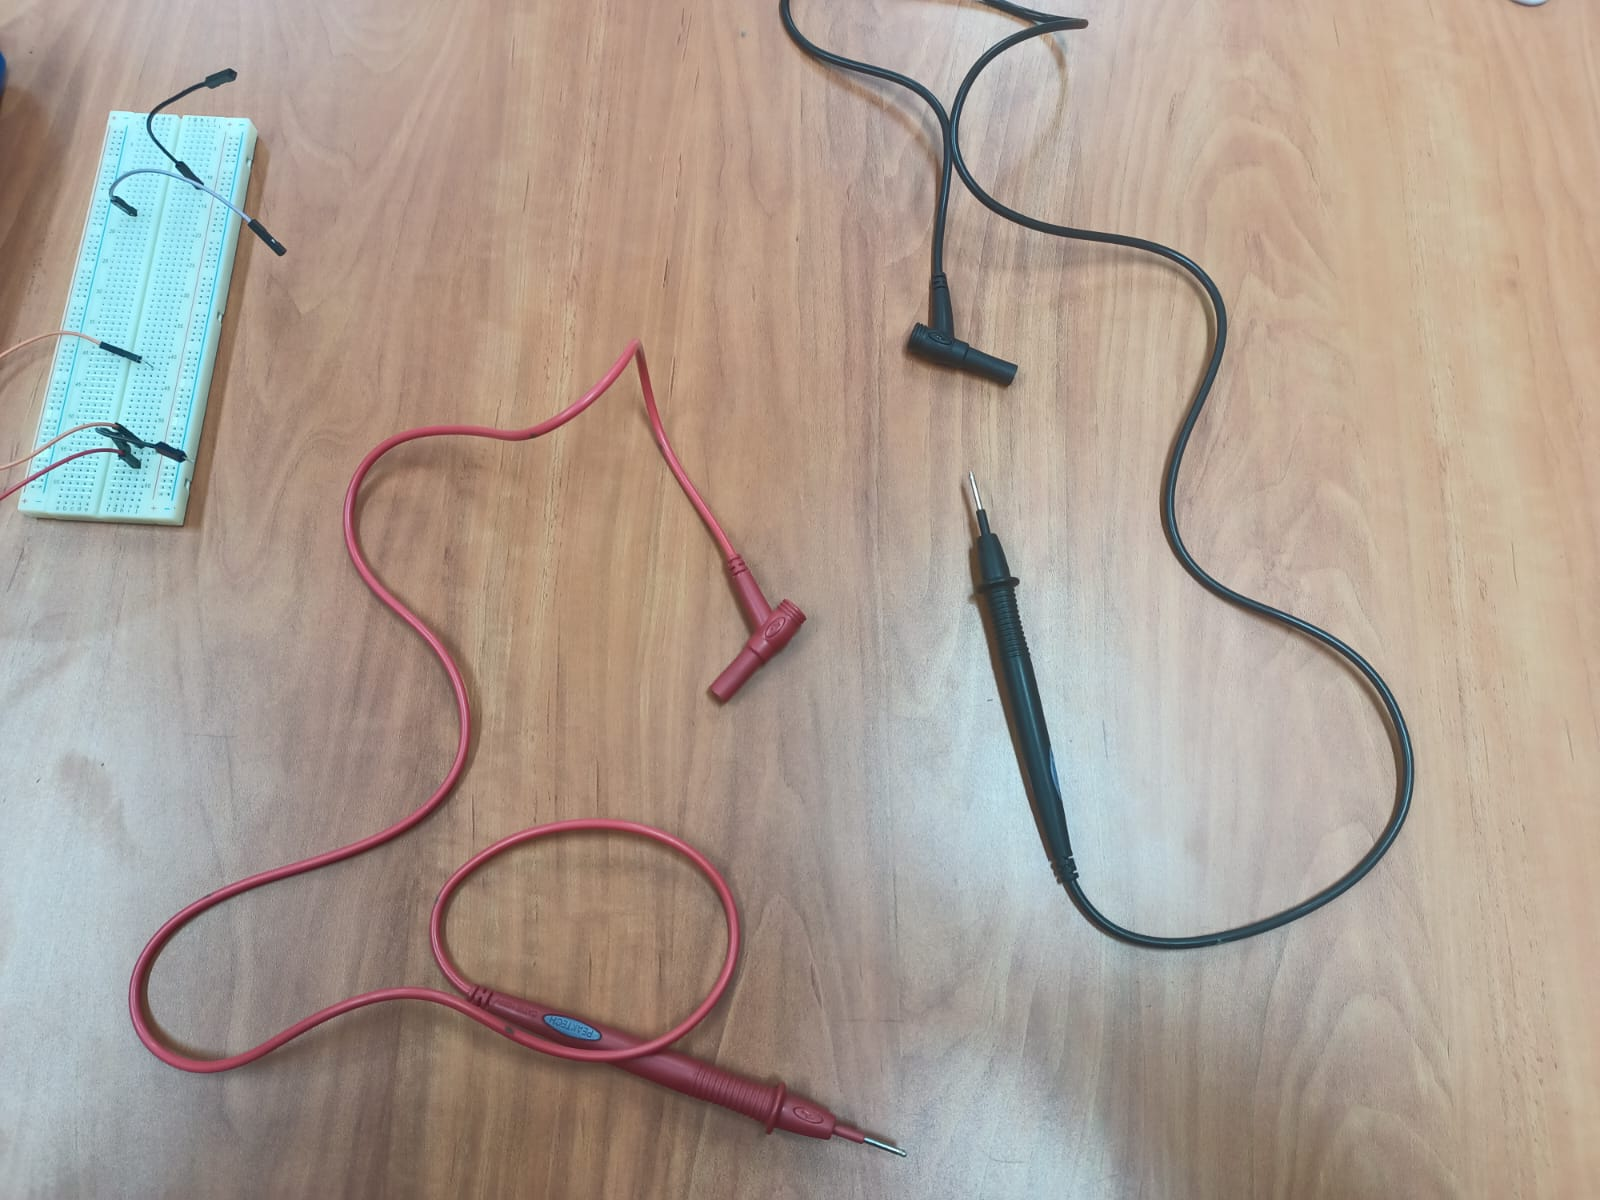
\includegraphics[scale = 0.1]{Imagenes/Material/Puntas.jpeg}\\
	Puntas para multímetro.

	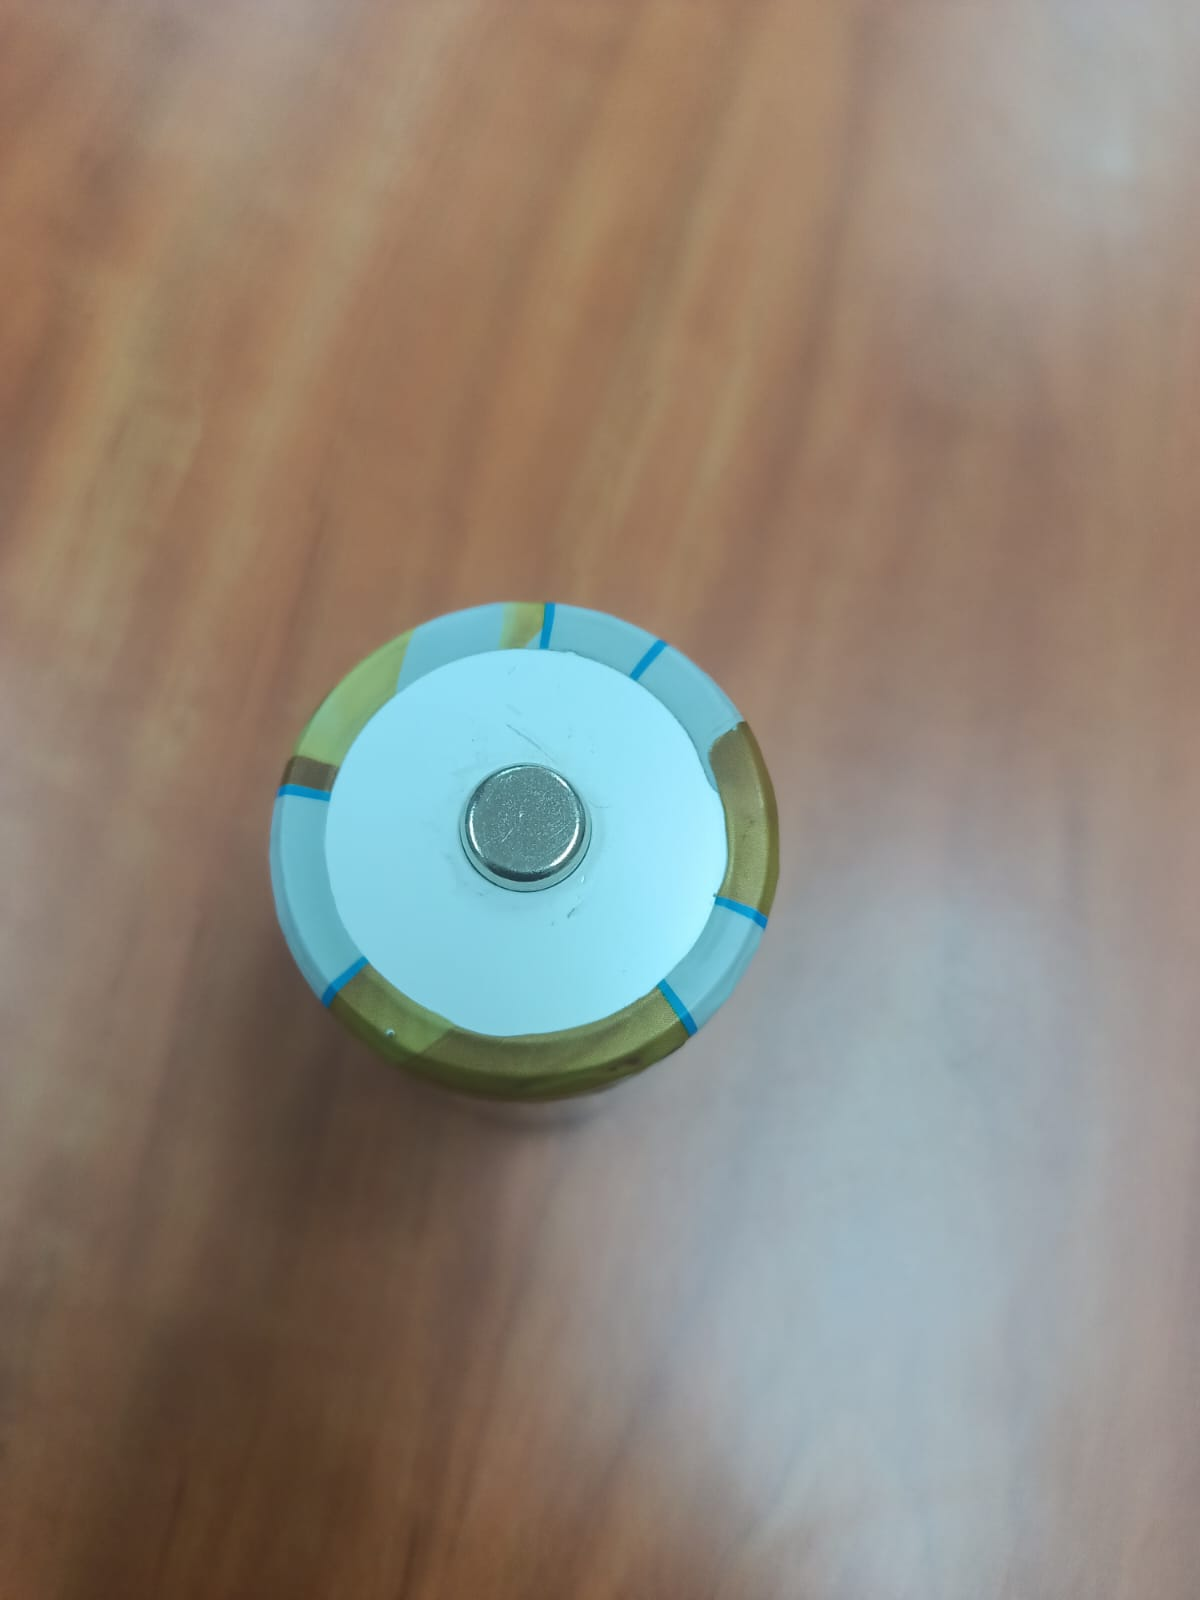
\includegraphics[scale = 0.1]{Imagenes/Material/PilaD.jpeg}\\
	Pila tipo "D" de 1.5 V.

	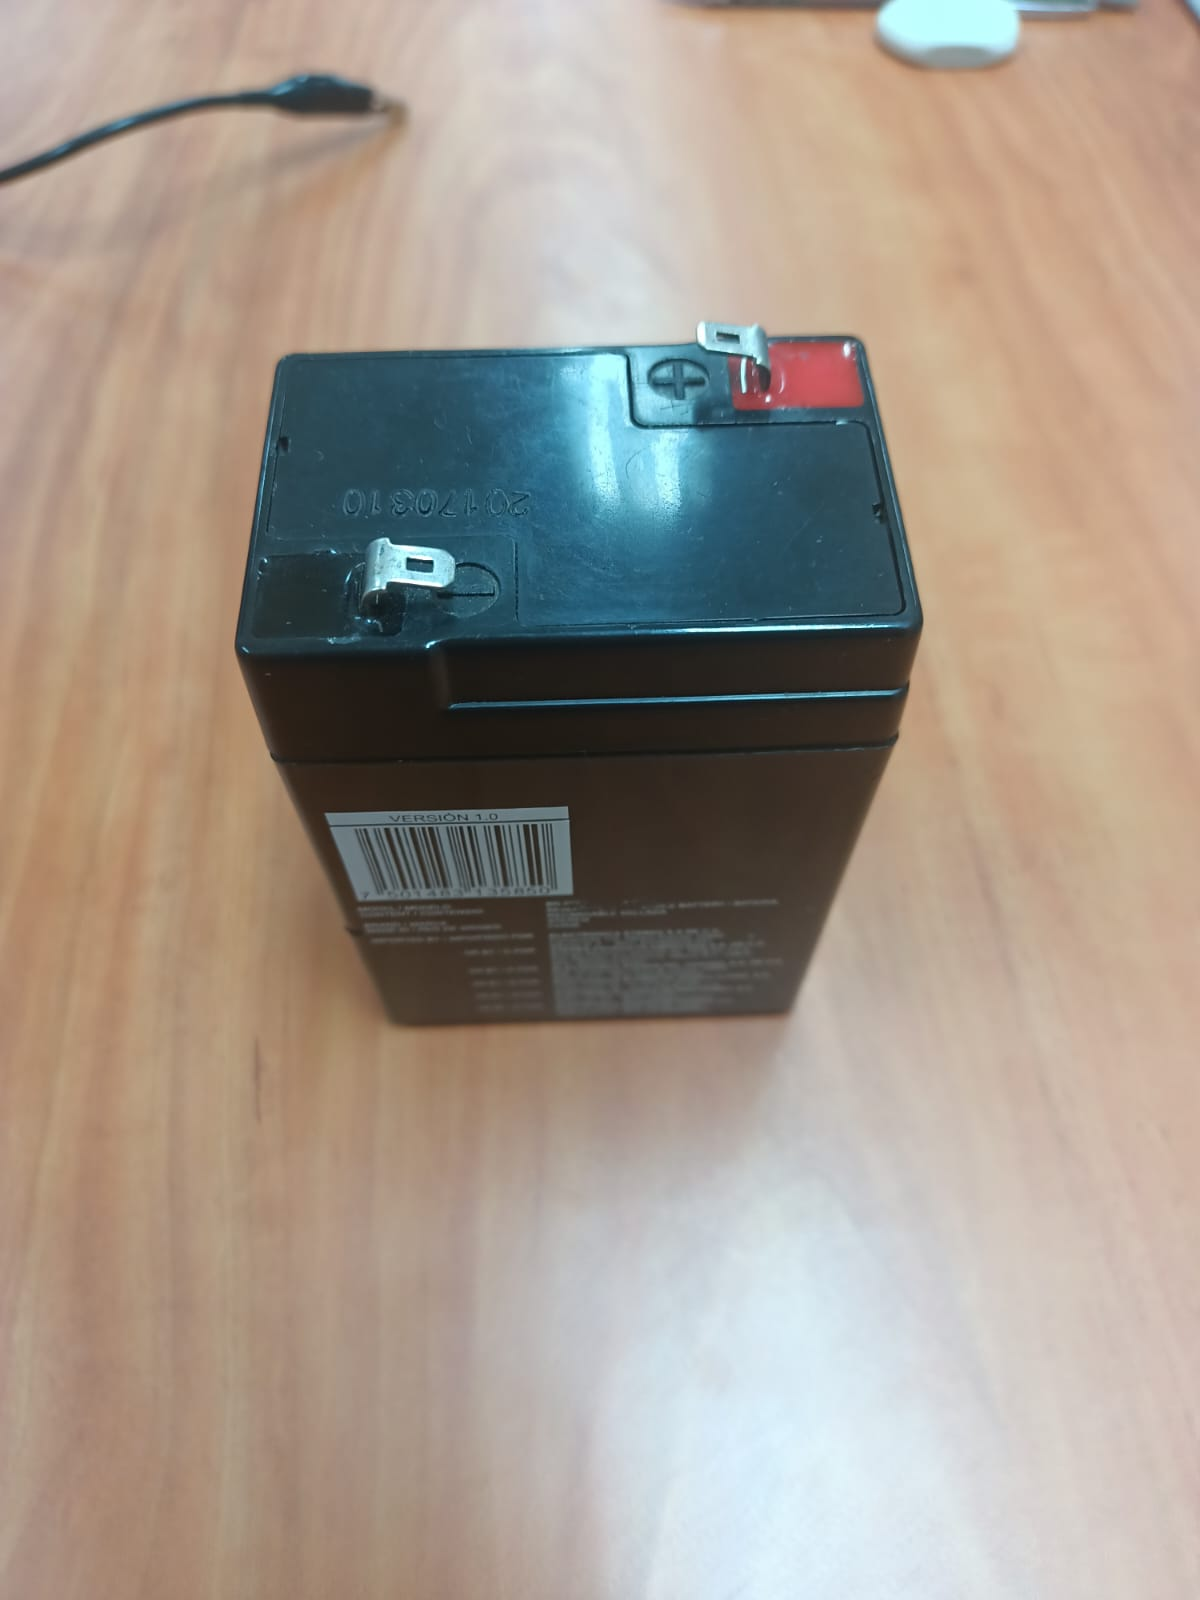
\includegraphics[scale = 0.1]{Imagenes/Material/PilaDes.jpeg}\\
	Pila de valor desconocido.

	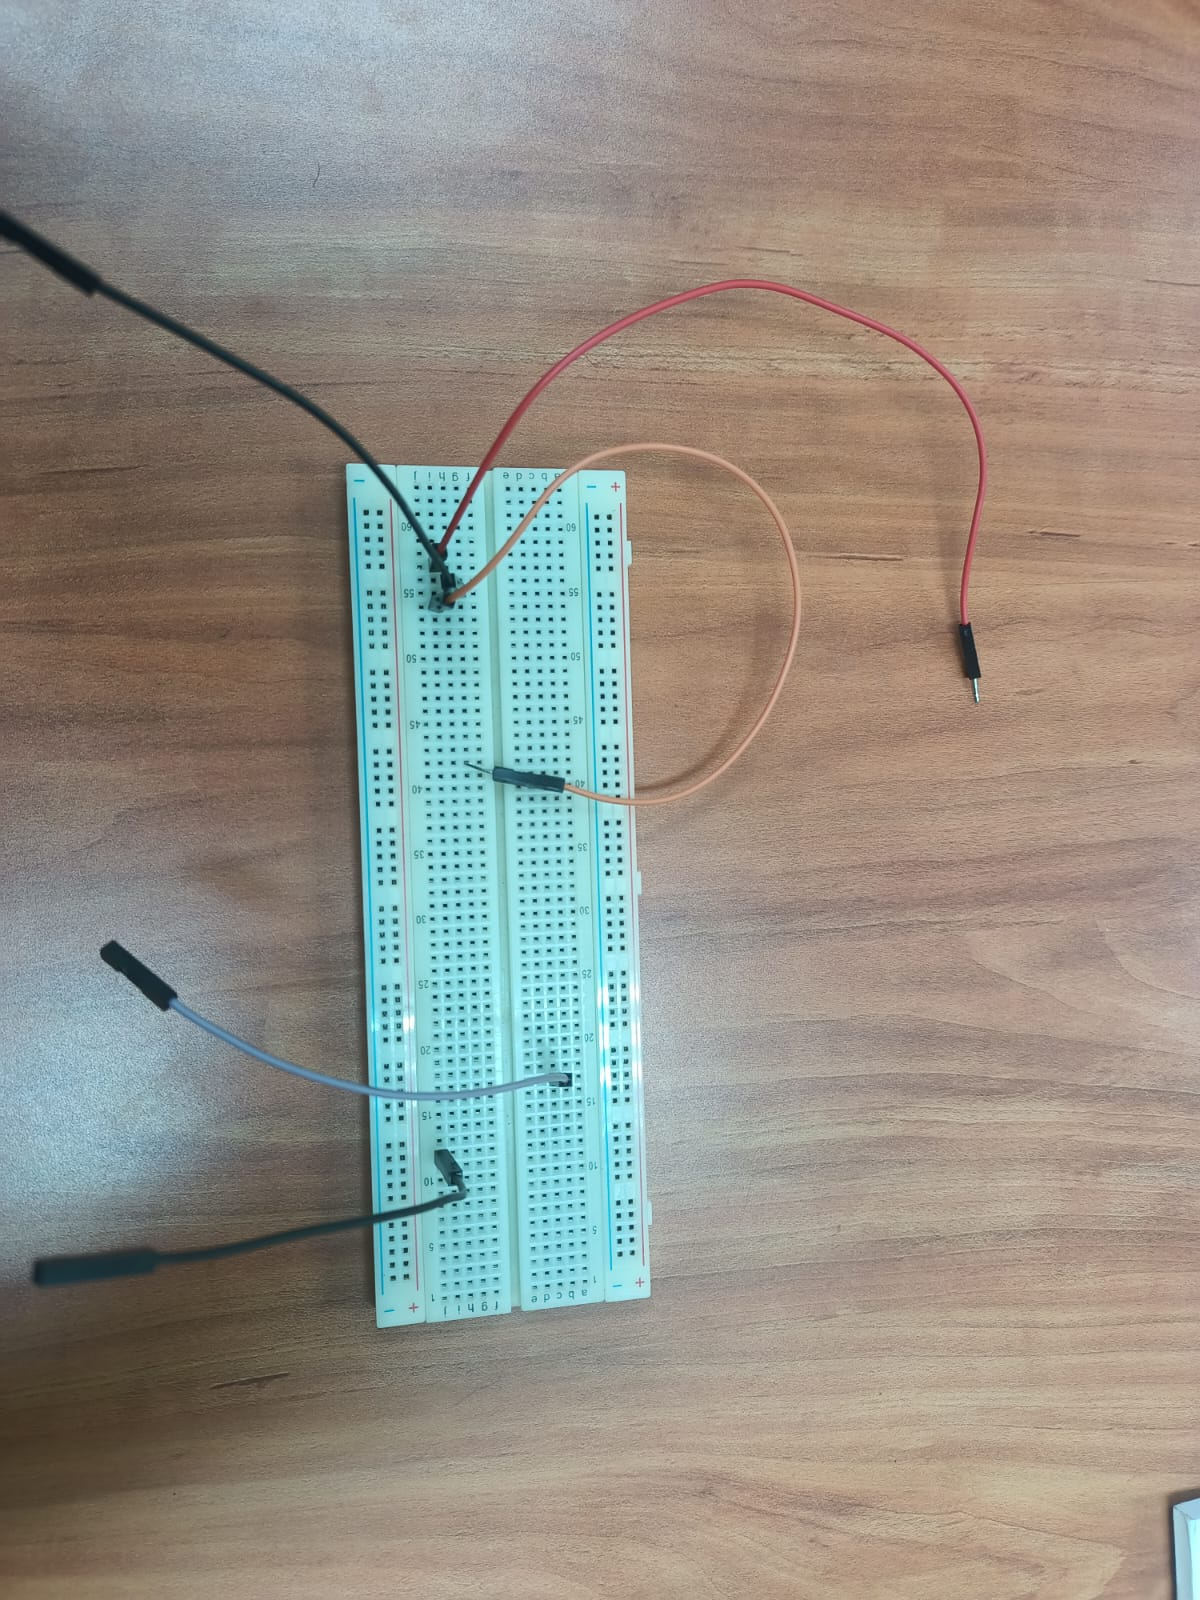
\includegraphics[scale = 0.1]{Imagenes/Material/Protoboard y jumper.jpeg}\\
	Protoboard y Jumpers.

	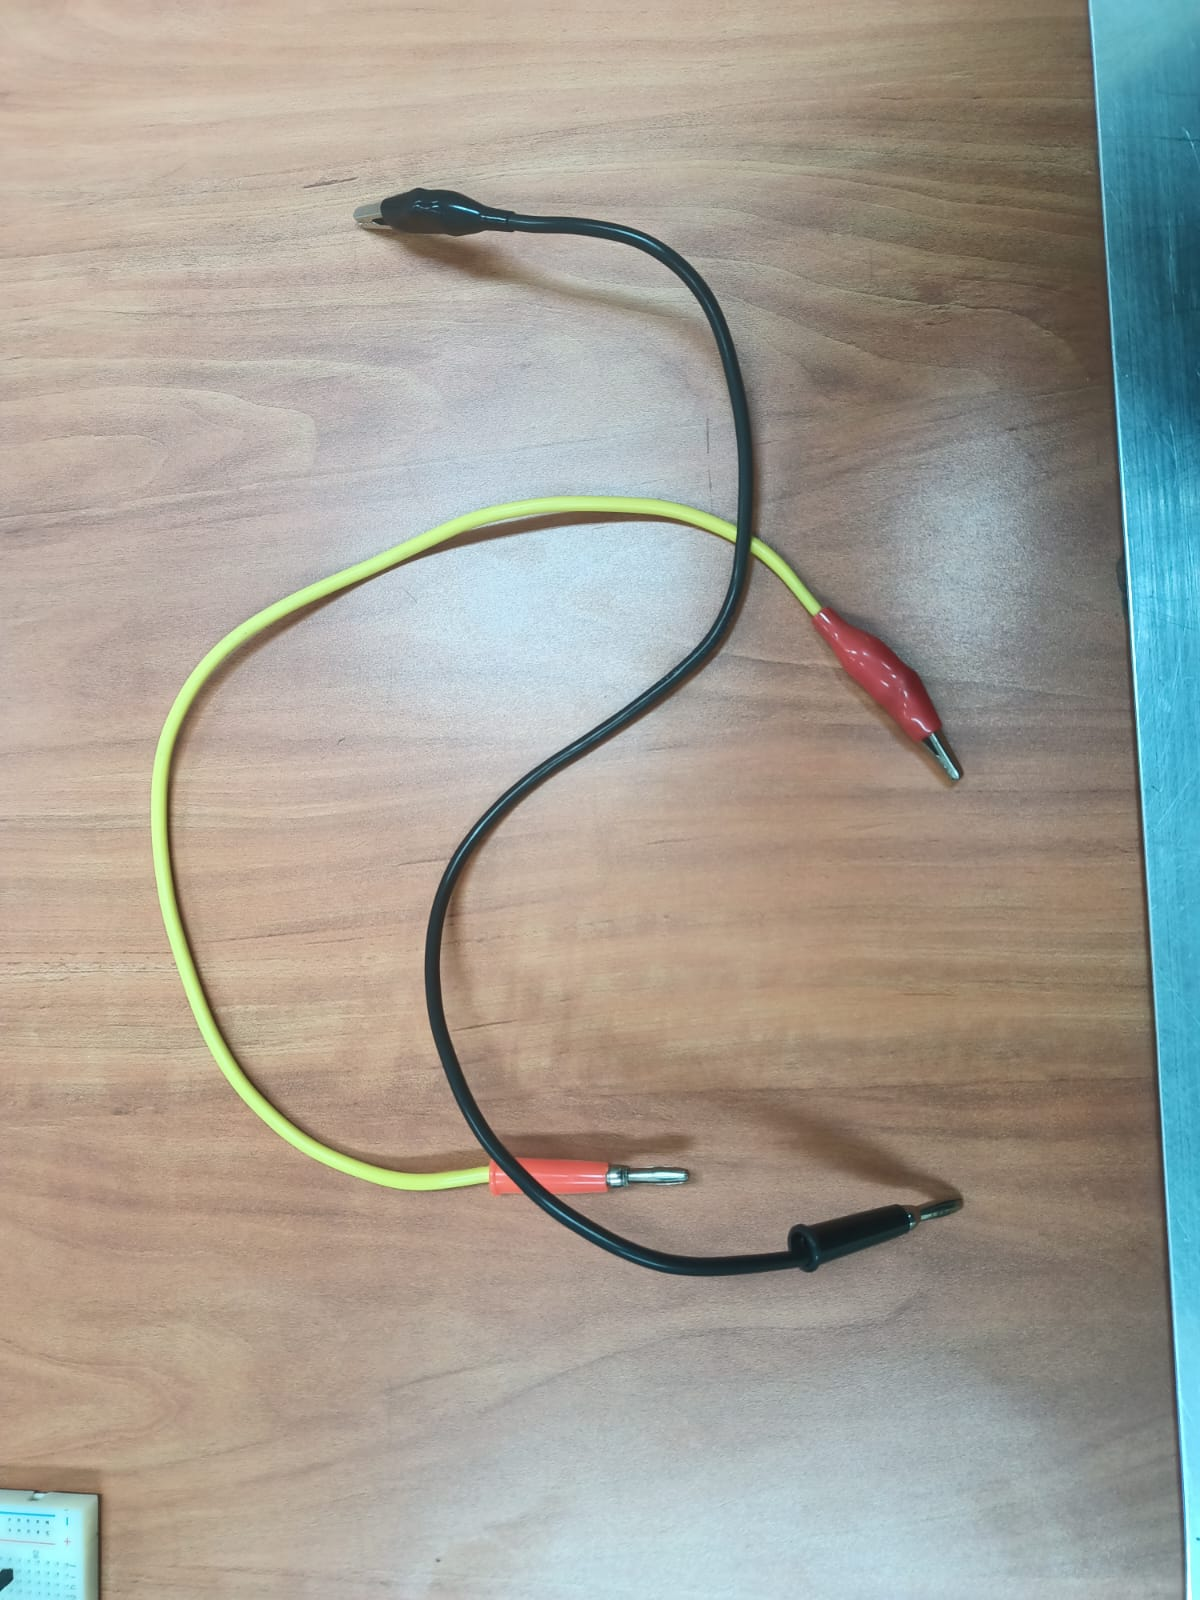
\includegraphics[scale = 0.1]{Imagenes/Material/Caimanban.jpeg}\\
	Cables <<Caimán-Banana>>.

	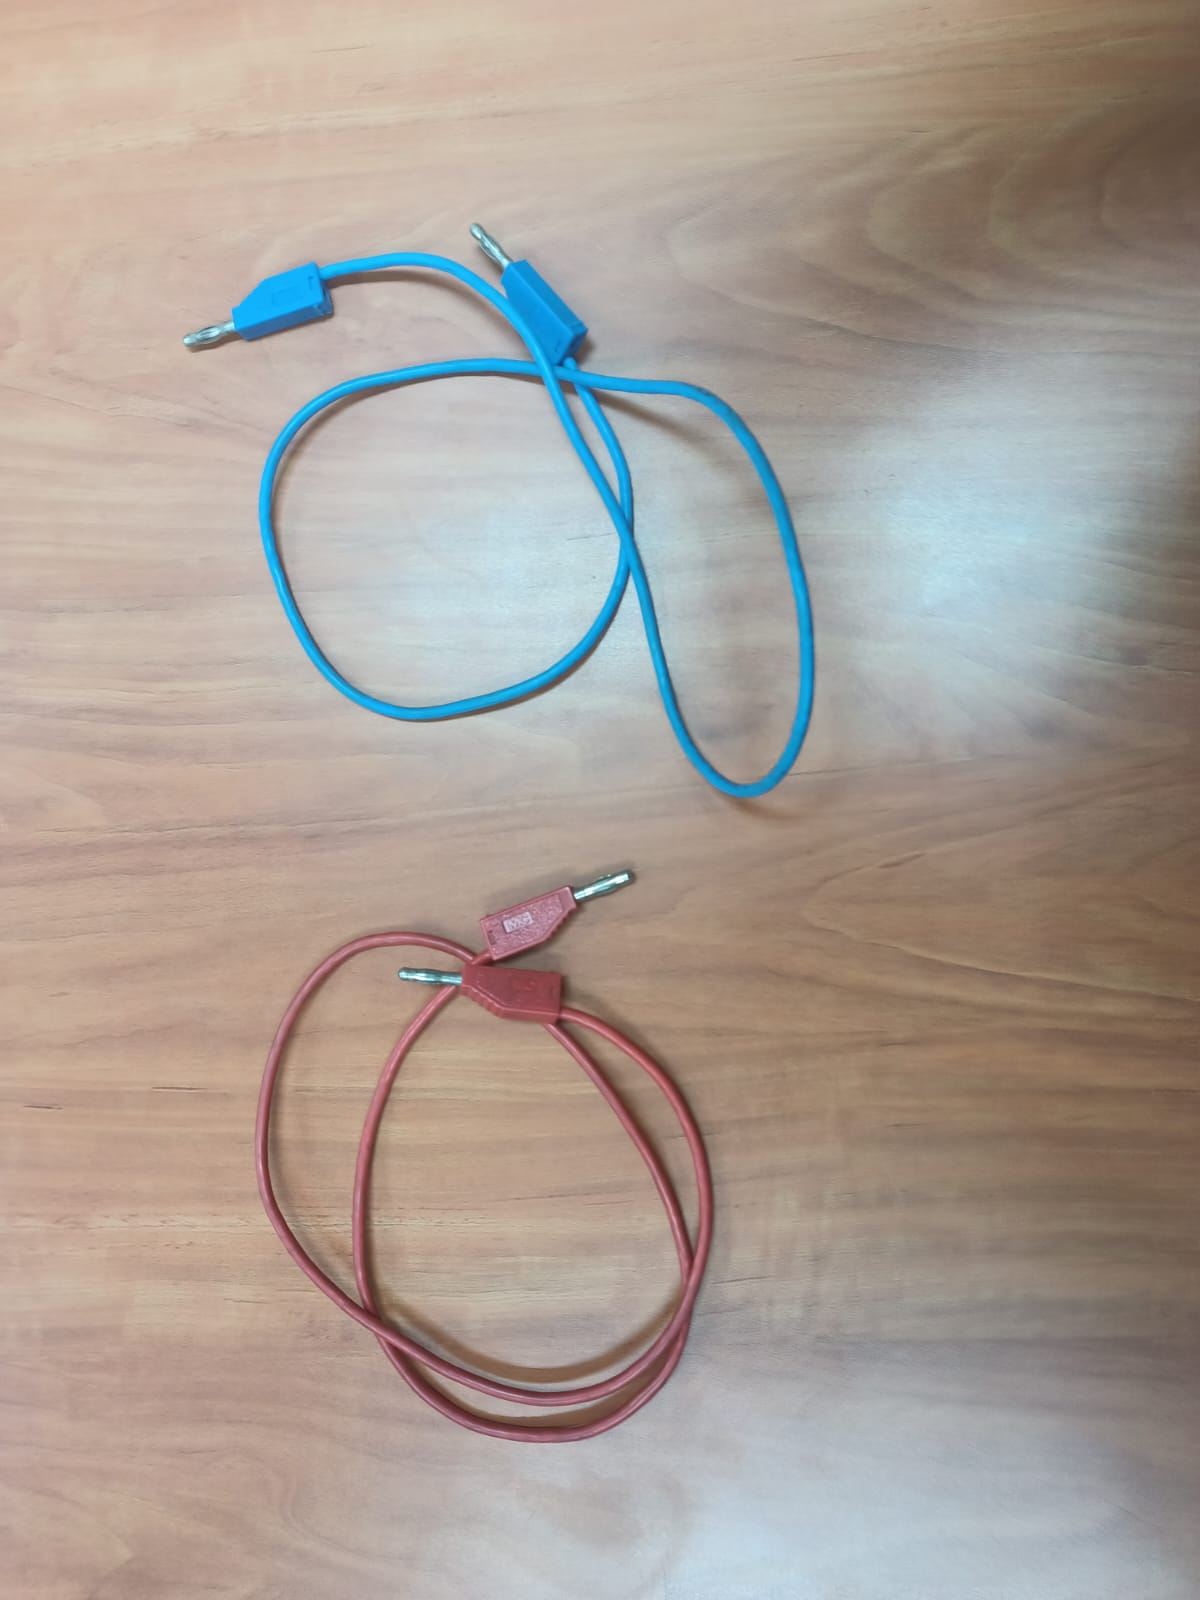
\includegraphics[scale = 0.1]{Imagenes/Material/banban.jpeg}\\
	Cables <<Banana-Banana>>.

	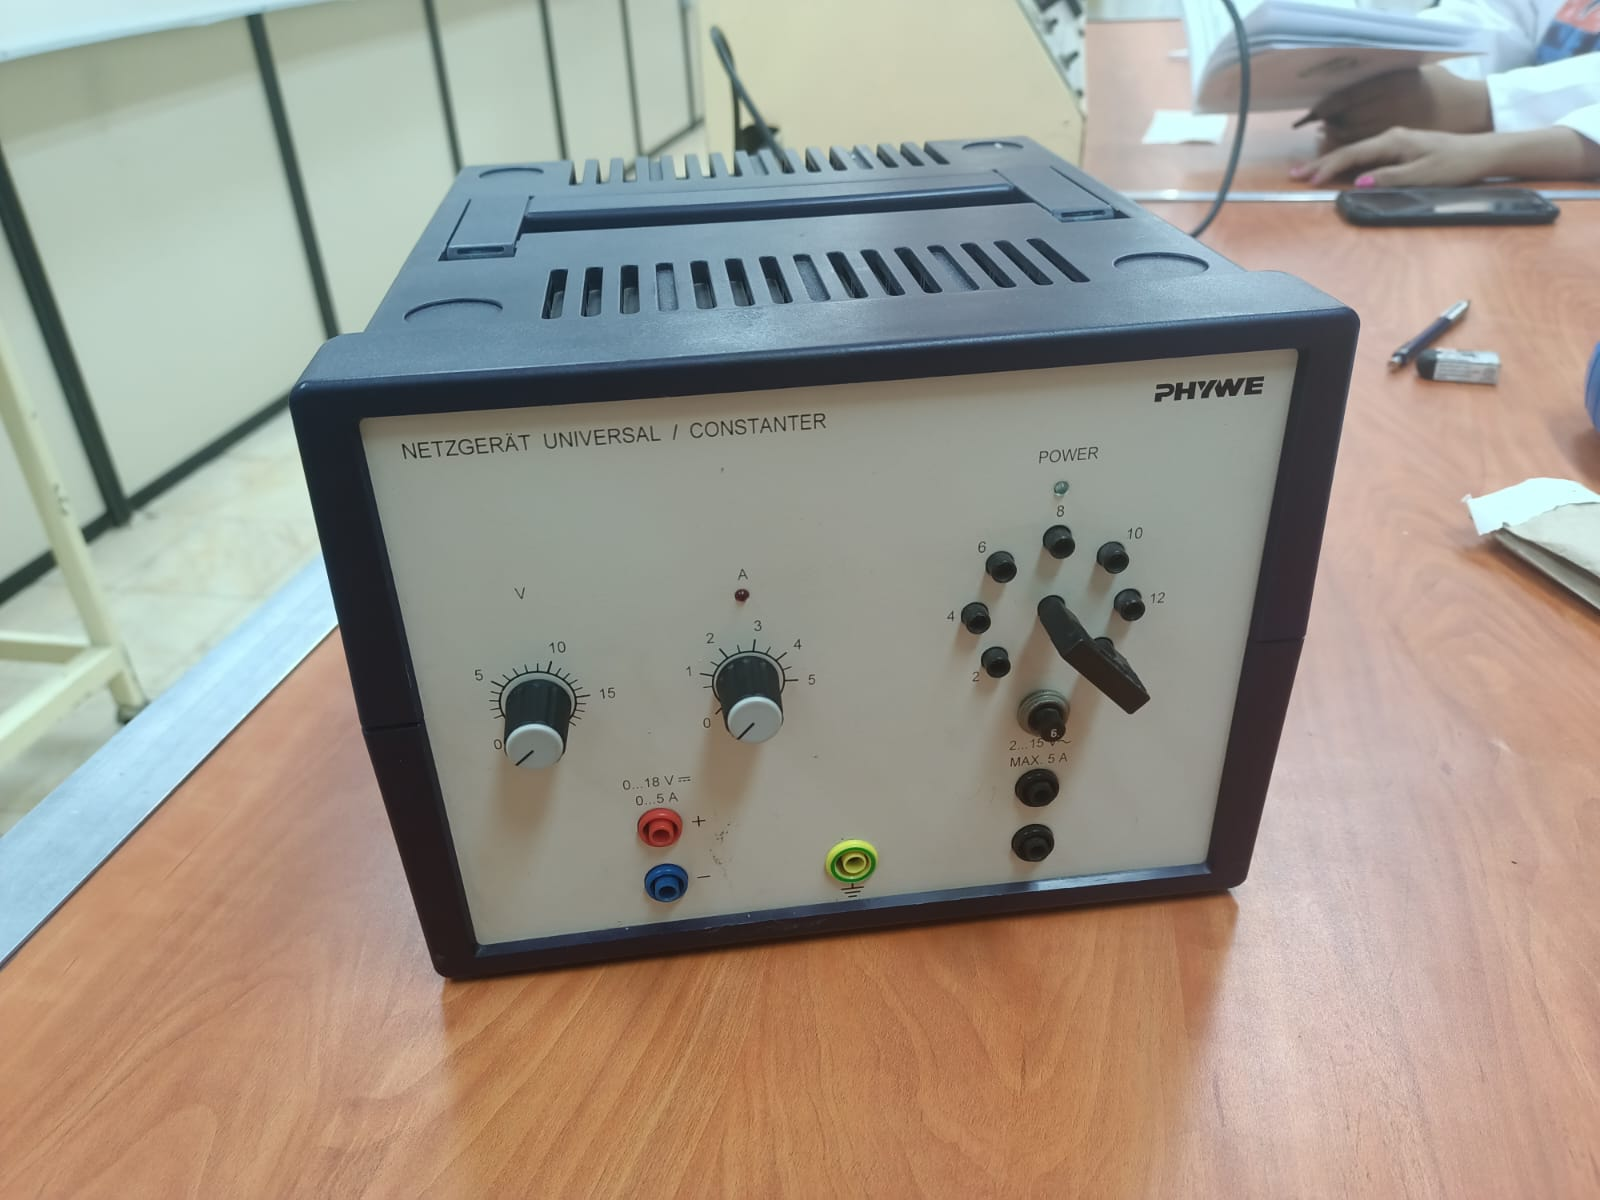
\includegraphics[scale = 0.1]{Imagenes/Material/FuenteVariable.jpeg}\\
	Fuente de alimentación regulada.

	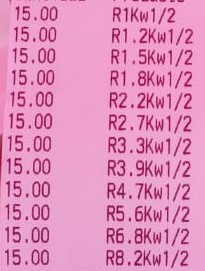
\includegraphics[scale = 1]{Imagenes/Material/Resistencias.jpeg}\\
	Resistencias de valores entre 1K$\Omega$ y 9K$\Omega$

\end{center}


\section{Desarrollo experimental.}

\subsection{Reconocimiento del multímetro.}

Tome el multímetro digital y reconozca lo siguiente:
\begin{enumerate}
	\item La marca y modelo del multímetro.
	\item Como encender el multímetro.
	\item Cuántas posiciones y cuáles son los rangos del multímetro para medir voltajes de Corriente Directa.
	\item Cuántas posiciones y cuáles son los rangos del multímetro para medir corrientes de Corriente Directa y Corriente Alterna.
	\item Cuántos y cuáles son los rangos del multímetro para medir resistencia.
	\item Otras funciones,interruptores y selectores.
\end{enumerate}

\subsection{Mediciones de resistencia(óhmetro).}

\begin{enumerate}
	\item Encienda el multimetro y coloque la perilla en Ohms.
	\item Anote los valores utilizando el código de colores para resistores.
	\item Mida los resistores y anote los valores obtenidos en una tabla.
	\item Compare el valor nominal con el valor medido.
\end{enumerate}

\subsection{Mediciones de continuidad.}

\begin{enumerate}
	\item Utilizando el medidor de continuidad o en la escala de resistencia más baja identifique como está constituida una protoboard.
	\item Elabore un diagrama según lo observado.
\end{enumerate}

\subsection{Mediciones de voltaje(vóltmetro).}

\begin{enumerate}
	\item Coloque la perilla del multímero en volts y ubique correctamente el selector de tipo de corriente en Corriente Directa.
	\item Mida el voltaje de las pilas y anote sus valores.
	\item Utilice la fuente regulada, ubique las salidas de corriente directa y realice tres mediciones diferentes respetando la polaridad.
\end{enumerate}

\subsection{Mediciones de voltaje de corriente alterna(vóltmetro).}

\begin{enumerate}
	\item Ubique un contacto como el mostrado en la siguiente imagen.\\
	\begin{center}
		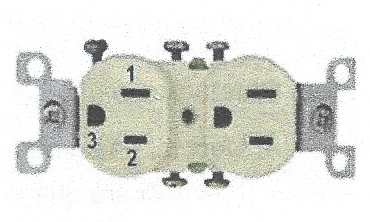
\includegraphics{Imagenes/Fotos/Contacto.png}
	\end{center}
	\item Mida el voltaje entre salidas y anote su valor.
	\item Identifique en el contacto cuál es la fase,el neutro y la tierra física.
\end{enumerate}

\subsection{Mediciones de intensidad de corriente continua(Amperímetro.)}
\begin{enumerate}
	\item Arme el siguiente circuito.\\
	\begin{center}
		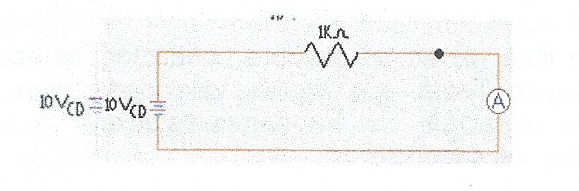
\includegraphics{Imagenes/Fotos/Circuito.png}
	\end{center}
	\item Seleccione una escala de medición adecuada y coloque el selector de Corriente Alterna y Corriente Directa en Corriente Directa.
	\item Mida la corriente en el circuito.
	\item Calcule el valor teórico de la corriente del circuito y compare con el valor medido.
\end{enumerate}

\section{Discusión de materiales .}


\section{Análisis y resultados.}

\subsection{Reconocimiento del multímetro.}

\subsection{Mediciones de resistencia(óhmetro).}

\subsection{Mediciones de continuidad.}

\subsection{Mediciones de voltaje(vóltmetro).}

\subsection{Mediciones de voltaje de corriente alterna(vóltmetro).}

\subsection{Mediciones de intensidad de corriente continua(Amperímetro.)}




\section{Conclusiones.}

\subsection*{Daniela Elizabeth Pérez Vargas.}

\subsection*{Jesús Martinez Amac.}
\subsection*{José Emilio Hernández Huerta.}

\subsection*{Nataly Bejarano Garduño.}
\subsection*{Uriel Grimaldi Díaz.}

\begin{thebibliography}{0}
	\bibitem{citekey}[Bragado, I. M. (2003). Física General.]
	\bibitem{citekey}[Benchimol, D. (c. 2020). Electrónica práctica. USERSHOP.]
	\bibitem{citekey}[Peaktech. (2016). Manual de Usuario Peaktech 2005.]
		
\end{thebibliography}

\end{multicols}

\end{document}
